\begin{center}
  \textbf{\Huge Slutinlämning}\\[1cm]
\end{center}
\section{Implementationsbeskrivning}
{\color{red}Den här sektionen använder ni för att beskriva hur projektet är strukturerat och implementerat. Algoritmer och övergripande design passar också in i det här kapitlet (bilder, flödesdiagram, osv. kan vara användbart). Skapa gärna egna delkapitel för enskilda delar, om det underlättar.\\ }
\subsection{Milstolpar}
{\color{red}``Ange för varje milstolpe om ni har genomfört den helt, delvis eller inte alls.  (Detta är främst till för att labbhandledaren ska veta vilken funktionalitet man måste ”leta efter” i koden.  Själva bedömningen beror inte på antalet milstolpar i sig.)''\\}
Den största ändringen från de planerade funktionerna är att projektet nu inte är modulärt. Efter att vi arbetat länge med strukturen av projektet så valde vi att börja om från början. Detta på grund av att det är väldigt komplicerat att skapa ett projekt som ska vara helt modulärt utan att t.ex. använda sig av så kallade ``Entity Systems''(\url{http://t-machine.org/index.php/2007/09/03/entity-systems-are-the-future-of-mmog-development-part-1/}.\\
\subsection{Dokumentation för programkod}
{\color{red}Programkod behöver dokumenteras för att man ska förstå hur den fungerar och hur allt hänger ihop.  Vissa typer av dokumentation är direkt relaterad till ett enda fält, en enda metod eller en enda klass och placeras då lämpligast vid fältet, metoden eller klassen i en Javadoc-kommentar, inte här.  Då är det både enklare att hitta dokumentationen och större chans att den faktiskt uppdateras när det sker ändringar.  Annan dokumentation är mer övergripande och placeras då här.  Det kan gälla till exempel:\\}
{\color{red}Övergripande programstruktur, t.ex. att man har implementerat ett spel som styrs av timer-tick n gånger per sekund där man vid varje sådant tick först tar hand om input och gör eventuella förflyttningar för objekt av typ X, Y och Z, därefter kontrollerar kollisioner vilket sker med hjälp av klass W, och till slut uppdaterar skärmen.\\}
\vspace{11pt}
{\color{red}Översikter över relaterade klasser och hur de hänger ihop.  Här kan det ofta vara bra att använda UML-diagram för att illustrera – men fundera då först på vilka grupper av klasser det är ni vill beskriva, och skapa sedan ett UML-diagram för varje grupp av klasser (det är sällan särskilt användbart att lägga in hela projektet i ett enda gigantiskt diagram).  Skriv sedan en textbeskrivning av vad det är ni illustrerar med UML-diagrammet.  Texten är den huvudsakliga dokumentationen medan UML-diagrammet hjälper läsaren att förstå texten och få en översikt.  IDEA kan hjälpa till att göra klassdiagram som ni sedan kan klippa och klistra in i dokumentet.\\}
\vspace{11pt}
{\color{red}Labbhandledaren och examinatorn kommer bland annat att använda den här dokumentationen för att förstå programmet vid bedömningen.  Ni kan också tänka er att ni själva ska vidareutveckla projektet efter att en annan grupp har utvecklat grunden.  Vad skulle ni själva vilja veta i det läget?  Om viktig information saknas kan ni få komplettera.\\}
{\color{red}När ni pratar om klasser och metoder ska deras namn anges tydligt (inte bara ”vår timerklass” eller ”utritningsmetoden”).\\}
{\color{red}Framhäv gärna det ni själva tycker är bra lösningar eller annat som handledaren borde titta på vid bedömningen.\\}
{\color{red}Se även sidan om krav på programkod på webben.\\}
{\color{red}Vi räknar med att de flesta projekt behöver runt 2-5 sidor för det här avsnittet.\\}
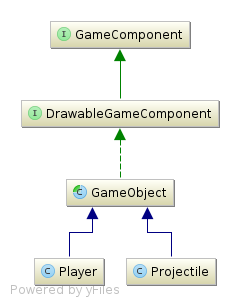
\includegraphics[scale=0.5]{gameobject}\\
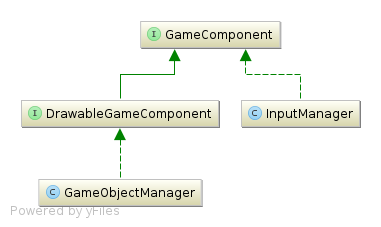
\includegraphics[scale=0.5]{managers}\\
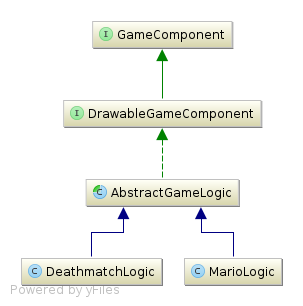
\includegraphics[scale=0.5]{gameLogics}\\
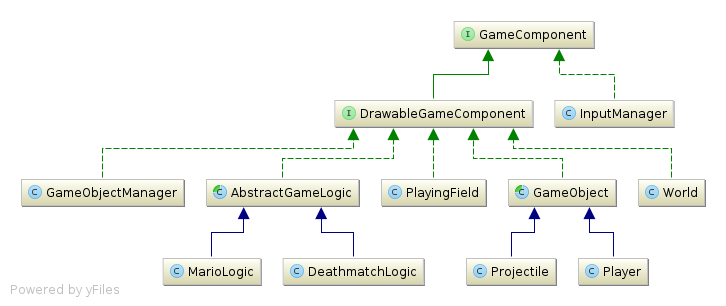
\includegraphics[scale=0.4]{all_gamecomponents}\\
\subsection{Användning av fritt material}
{\color{red}Skriv ner vilka klassbibliotek och vilket annat fritt material ni har använt utöver det som ingår i Java 7, eller ange uttryckligen att ni inte har använt något.\\}
Vi har använt oss av klassbiblioteket Slick2D för utritning av spelet. Slick2D är i sin tur baserat på klassbiblioteket LWJGL som är en java wrapper för OpenGL.
\subsection{Användning av designmönster}
{\color{red}Beskriv tydligt i numrerad lista vilka designmönster som använts i implementationen, vad ni åstadkommer genom att använda just de designmönstren i just ert projekt (vad var bra med att använda det?), och hur designmönstret har realiserats i praktiken, t.ex. vilka klasser som är inblandade och vad de motsvarar i designmönstrets terminologi (”Klasserna X och Y är våra konkreta strategier för den här användningen av strategimönstret”).\\
Beskrivning från websidan:\\
\begin{tabular}{| p{11cm} |}
    \hline
    För varje betygsnivå måste ett visst antal designmönster implementeras och användas, för att ni ska visa att ni behärskar dem. Designmönstren måste användas på ett lämpligt sätt, dvs. varje mönster måste användas för att implementera funktionalitet där det mönstret faktiskt passar. Detta kan till viss del påverka vilken funktionalitet ni implementerar. \\ \hline
    Designmönstren ska implementeras från grunden. Om ni använder en Comparator som argument till Javas sorteringsmetoder räknas det inte som att ni har implementerat Strategy-mönstret. \\ \hline
    Alla designmönster från Design Patterns av Gamma, Helm, Johnson och Vlissides är godkända. Fråga examinatorn om ni vill tillgodoräkna er andra mönster och ge en referens till det mönster ni undrar över. \\ \hline
    Beskriv noggrant var och hur designmönstret är implementerat (vilka klasser/metoder i er kod), varför ni valde att använda detta mönster snarare än något annat mönster eller en ad-hoc-metod, samt en kortare förklaring av designmönstrets för- och nackdelar i denna specifika situation. \\ \hline
\end{tabular}\\}
\vspace{11pt}
1. Factory Method\\
Detta mönster är uppbygt utav ett interface eller en funktion som returnerar en ny instans utav ett objekt givet ett visst antal parametrar, till skilland från att direkt skapa ett objekt så kan dessa funktioner själva lägga till information till extra information till objektet som anroparen inte skulle kunnat göra utan att bryta mot abstraktionen.\\
World.spawnNewPlayer givet en spelarfärg skapar en ny spelare, hittar en fri position på kartan och lägger till spelaren till spelet.\\
ResourceLoader klassen som givet ett filnamn laddar in en resurs av en viss typ. En ResourceLoader instans är bunden till en viss typ av resurs. En TiledMapLoader laddar in ett TiledMap objekt osv\ldots ResourceManager klassen hanterar bindningen mellan resurstypen och laddaren.\\
\vspace{11pt}
2. Builder Pattern\\
Detta mönster är uppbygt av två delar. Själva direktorn som håller reda på byggarna(``Builders'') och en eller flera byggare som själva skapar objekt. Man kan se direktorn som en proxy för byggarna.\\
ResourceManager är i detta fall klassen som är direktorn och hanterar valet av vilken ``builder'' som ska väljas för inladdning av resursen. Själva ``builder'' interfacet är i detta fall ResourceLoader som implementeras av till exempel TiledMapLoader. ResourceManager har även en objektcache så att den inte laddar om samma objekt flera gånger.\\
\subsection{Användning av objektorientering}
{\color{red}För varje betygsnivå måste ni peka ut ett visst antal lösningar ni har gjort där ni använder objektorienterade "finesser" som t.ex. polymorfism.  Diskutera hur man kunde ha löst detta utan objektorientering och kontrastera de lösningarna mot varandra. \\
Beskrivning från websidan:\\
\begin{tabular}{| p{11cm} |}
    \hline
    För varje betygsnivå måste ni peka ut ett visst antal lösningar ni har gjort där ni använder objektorienterade "finesser" som t.ex. polymorfism, och diskutera kortfattat (några meningar) hur man kunde ha löst detta utan objektorientering. \\ \hline
    Tänk på att det verkligen ska gälla finesser som är "unika" för objektorientering. Enum-konstanter finns t.ex. i olika former i icke-OO-språk som C. Serialisering av datastrukturer finns också i icke-OO-språk. \\ \hline
\end{tabular}\\}
\vspace{11pt}
1. Polymorphism\\
GameObject klassen är en abstrakt klass som representerar alla objekt på spelplan. Klasserna Player och Projectile ärver och utökar GameObject.\\
GameObjectManager klassen lagrar alla aktiva instanser utav GameObject klassen.\\
\vspace{11pt}
2. Enums är Objekt (i Java)\\
Detta går även att implementera i andra språk än Java med då med statiska fält i klasser.
Vi använder oss av att enums i java är objekt genom att använda detta för att lagra egenskaper för spelet/kartan (Se PlayingField.Options).\\
En enum i Java är egentligen en klass med statiska fält med instanser utav klassen, och när man skickar enums som parametrar så skickar man dessa instanser. Jämförelse görs enkelt eftersom == operatorn jämför minnesadresser.\\
Tack vare våran implementation av Options så kan vi enkelt och snyggt beskriva egenskaper och dess standardvärden. Och även enkelt ändra värden på dessa egenskaper utan att använda en Map eller liknande för lagring.\\
\vspace{11pt}
3. Interfaces\\
Vi använder interfaces i flera delar av spelet. Bland de viktigaste interfacen är GameComponent, som beskriver en del av spelet som kan initieras, updateras och tas bort. En utökning av detta interface är DrawableGameComponent som även har en funktion för utritning.\\
Dessa interface implementeras utav alla spelobjekt(GameObject) men även av andra viktiga klasser som GameObjectManager, InputManager och AbstractGameLogic.\\
\subsection{Motiverade designbeslut med alternativ}
{\color{red}Här anger ni (numrerade) motiverade designbeslut enligt betygskraven på webben.  Anledningen är både att ni ska visa oss hur ni har tänkt och att ni själva ska fundera och reflektera över era val.\\
Sådant som ska göras enligt projektkraven är inte (gruppens) designbeslut, t.ex. att de flesta fält ska vara privata.  De alternativa lösningarna som ni anger ska vara någorlunda rimliga (det är normalt inte ett designbeslut att dela upp koden i flera klasser eftersom alternativet för ett projekt av den här storleken skulle vara absurt).\\
Beskrivning från websidan:\\
\begin{tabular}{| p{11cm} |}
    \hline
    För varje betygsnivå måste ni beskriva ett visst antal designbeslut ni har tagit, med särskild tonvikt på användning av objektorientering. För varje designbeslut ska ni beskriva vad ni ville åstadkomma, hur ni gjorde, minst en annan alternativ lösning, och varför den lösning ni gjorde var bättre än alternativet. (I vissa fall kanske ni inser att den lösning ni valde var sämre än alternativet – beskriv då varför.) Detta ska vara andra lösningar än de som kommer från punkten ovan. \\ \hline
    Designbesluten ska vara på rimligt hög "objektorienterad nivå", dvs. inte varför ni valde att använda "int" istället för "long" för ett visst fält... Använde ni en enda lyssnarklass för knapparna i ett GUI, eller flera? Använder ni fabriker, prototyper eller vanliga konstruktorer för att skapa brickor i Breakout? \\ \hline
\end{tabular}\\}
\vspace{11pt}
1. \ldots \\
2. \ldots \\
3. \ldots \\
4. \ldots \\
5. \ldots \\
6. \ldots \\
7. \ldots \\
8. \ldots \\
\section{Användarmanual}
{\color{red}När ni har implementerat ett program krävs det också en manual som förklarar hur programmet fungerar. Ni ska beskriva programmet tillräckligt mycket för att en labbhandledare själv ska kunna starta det, testa det och förstå hur det fungerar. \\}
\vspace{11pt}
LWJGL (Lightweight java-game library) och slick2d är dependencies.\\
Kontrollerna är hårdkodade i inputManager-klassen (planerade feature att lägga detta i en konfigurationsfil) och är för nuvarande\\
Spelare 1:\\
Sikta motsols: W\\
Sikta medsols: S\\
Vänster: A\\
Höger: D\\
Skjut: G\\
Hoppa: H\\
\vspace{11pt}
Spelare 2:\\
Sikta motsols: upp\\
Sikta medsols: ned\\
Vänster: vänster\\
Höger: höger\\
Skjut: Ins (numpad 0 med num lock avslaget)\\
Hoppa: Del (numpad , med num lock avslaget)\\
\vspace{11pt}
Men dessa går såklart att ändra i källkoden. Lista över tillgängliga knappar finns på \url{http://www.java-gaming.org/index.php?topic=27994.0}.\\
\vspace{11pt}
\vspace{11pt}
Även namnet på kartfilen är hårdkodat, i World-klassen. Detta är också planerat att läggas i en konfigurationsfil och är för nuvarande default.tmx .\\
För att ändra och skapa kartfiler används Tiled ( \url{http://www.mapeditor.org/} ) och inställningar för gravitation, friktion etc kan ställas in där.\\
\vspace{11pt}
<insert instructions for tiled>\\
<is there even any settings being changed in the mapfile? At least change MAPNAME and AUTHOR>\\
\vspace{11pt}
Ovanför varje spelare finns en health bar, som krymper när man tar skada. Man tar skada genom att träffas av skott <samt bli hoppad på?>. När mätaren når botten förlorar man ett liv och spelaren återskapas på en slumpmässig plats på kartan. Siffran till vänster om mätaren är antalet liv man har kvar (alt. antalet gånger man kan återskapas). När man dör med 0 liv återskapas man inte och är ute ur matchen. När endast en spelare återstår tar spelet slut och vinnaren skrivs ut på skärmen. Sedan startar spelet om några sekunder senare.\\
\vspace{11pt}
Röd terräng är förstörbar och går sönder om man skjuter på den.\\
\vspace{11pt}
Man kan hoppa om man står på fast mark (röd, grön eller slutet på kartan). Det går även att "vägghoppa" (eng. wall jump) genom att nudda en vägg åt en sida, styra i motsatt riktning samt hoppa samtidigt, detta är dock ganska svårt att få till.\\
\vspace{11pt}
Inkludera flera (minst 3) skärmdumpar som visar hur programmet ser ut!\\
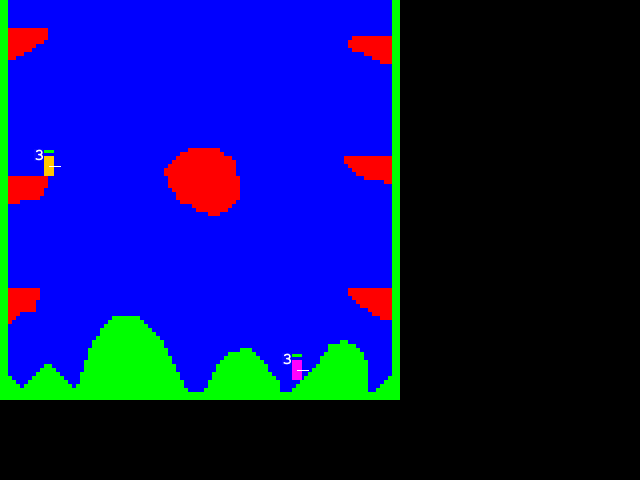
\includegraphics[scale=0.5]{game_1}\\
\vspace{11pt}
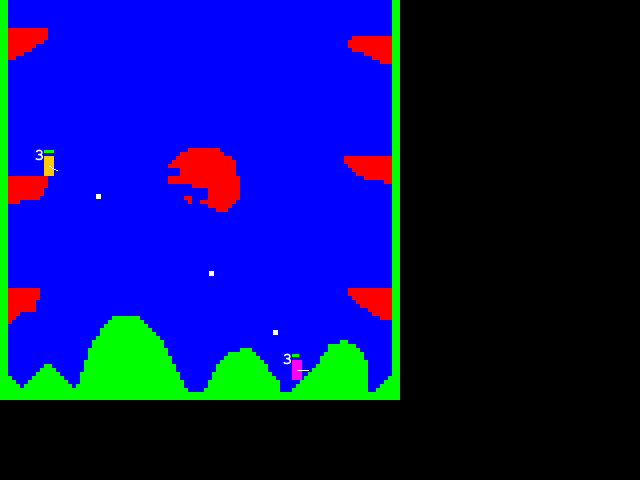
\includegraphics[scale=0.5]{game_2}\\
\vspace{11pt}
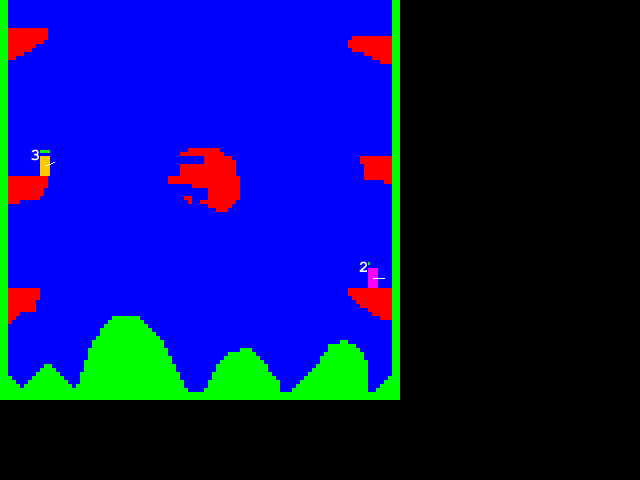
\includegraphics[scale=0.5]{game_3}\\
\vspace{11pt}
<mitten av spelet på en annan bana>\\
\vspace{11pt}
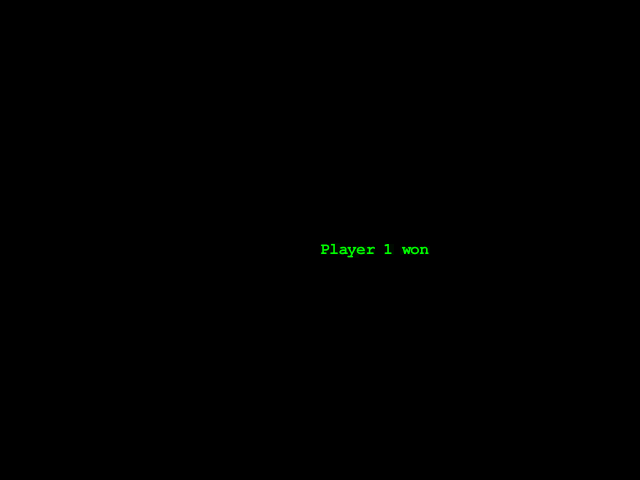
\includegraphics[scale=0.5]{game_5}\\
\section{Betygsambitioner}
{\color{red}Ange här vilket betyg ni siktar på i ert projekt.  Se sedan till att ni har följt de mätbara kraven för detta betyg och att detta finns dokumenterat i projektbeskrivningen ovan.\\}
\section{Utvärdering och erfarenheter}
{\color{red}Detta avsnitt är en väldigt viktig del av projektspecifikationen. Här ska ni tänka tillbaka och utvärdera projektet (något som man alltid bör göra efter ett projekt). Som en hjälp på vägen kan ni utgå från följande frågeställningar:\\
Vad gick bra? Mindre bra?\\

I början av projektet hade vi väldigt storslagna planer på hur vi skulle göra ett helt modulärt spel där användaren lätt skulle kunna byta ut centrala delar av programmet. Detta var dock mer än vi klarade av och vi spenderade mycket tid på att planera hur abstraheringen skulle se ut, dock inte tillräckligt och när vi satte oss ned för att programmera var det fortfarande många frågetecket kvar. Det slutade med att vi två veckor innan deadline knappt hade någon kod skriven och vi kom fram till att det inte skulle gå. Vi skippade majoriteten av all modularitet vilket gjorde abstraheringen mycket enklare, och kunde således koncentrera oss på att skriva koden. Det blev stressigt mot slutet men vi lyckades hinna klart med den grundläggande delen av spelet. 

Lade ni ned för mycket/lite tid?\\

De första veckorna la vi ned alldeles för lite tid, vilket bl.a. berodde på att det var så svårt att skriva och att man inte kom någonstans när man skrev, så det var inte kul att kod. De sista veckorna la vi ned mycket mer tid och gjorde stora framsteg vilket var kul. Sett på det stora hela så hade vi nog gärna lagt ned mer tid och implementerat mer funktioner.

Var arbetsfördelningen jämn? Om inte: Vad hade ni kunnat göra för att förbättra den?\\

Arbetsfördelningen var relativt jämn. Mikael gjorde nog lite mer då han är mer erfaren programmerare inom objektorientering och John hade assistentjobb och annat som hjälpte till att ta tid och ork ur honom.

Har ni haft någon nytta av projektbeskrivningen? Vad har varit mest användbart med den? Minst?\\

Vi har nog nästan inte haft någon nytta av projektbeskrivningen. Vi planerade nog lite mer och specade hur spelet skulle bli, men då vi kommunicerade mycket med varandra tittade vi sällan på projektbeskrivningen. 

Har arbetet fungerat som ni tänkt er? Har ni följt "arbetsmetodiken"? Något som skiljer sig? Till det bättre? Till det sämre?\\
Vad har varit mest problematiskt, om man utesluter den programmeringstekniska delen? Alltså saker runt omkring, som att hitta ledig tid eller plats att vara på.\\

Mest problematiskt har varit att finna motivation och tid. Då vi använt slick2d och lwjgl har vi heller inte kunnat koda och testa på skoldatorerna, men det har inte varit något större problem annat än på redovisningspass.

Vad har ni lärt er så här långt som kan vara bra att ta med till era egna kommande kurser/projekt?\\
Vilka tips skulle ni vilja ge till studenter i nästa års kurs?\\
Har ni saknat något i kursen som hade underlättat projektet?\\
\vspace{11pt}
Vi använder detta för att utveckla och förbättra kursen till nästa år.  Vissa delar som är användbara som tips till andra studenter kan komma att citeras (givetvis helt anonymt!) under föreläsningar eller på websidor.\\
(Glöm inte att exportera till PDF-format innan ni skickar in!)\\}
